\section{Auvi}

\subsection{Programm} % AuVi
Um Verwechslungen zu verhindern ist das Programm,
welches unter AuVi entwickelt wurde ,,\vs ''.
Der Kürzel steht für Visualisierung System und ist in verschiedenen Versionen lauffähig.
Die Aufgabe von \vs\ ist es auf eine Datenquelle zuzugreifen
und nach abgespeicherten Parametern die Rohdaten in Grafiken umzuwandeln.
Dabei wird sehr viel Wert darauf gelegt,
dass das Erstellen der Grafiken möglichst abstrakt behandelt wird,
damit der Nutzer sehr großen Einfluss auf das Design und den Inhalt der Grafiken nehmen kann.

\subsection{Meteorologie} % AuVi

\subsubsection{Prognosetheorie} % AuVi Meteorologie
Die Meteorologie gehört zu den Naturwissenschaften und
beschäftigt sich mit der Atmosphäre, der Wetterprognose und der Klimatologie \cite{meteorologie}.
Sie liefert somit die Voraussetzungen um eine Wettervorhersage erstellen zu können.
Unter einer Wetterprognose versteht man die Vorhersage eines Zustands
der Atmosphäre zu einem bestimmten Zeitpunkt an einem bestimmten Ort
oder in einem bestimmten Gebiet.
Es wird nicht nur das Wetter in Bodennähe betrachtet,
sondern auch Wettererscheinungen in höheren Schichten der Erdatmosphäre.
\\
Das Wetter lässt sich durch entsprechende Naturgesetze beschreiben.
Das ist für die Prognose essentiell wichtig.
Der Grundgedanke einer solchen Prognose besteht darin,
aus einem bereits vergangenen und dem aktuellen Zustand
der Atmosphäre einen Zustand in der Zukunft abzuleiten.
Dazu werden die bekannten physikalischen Regeln angewandt.
In mathematischer Hinsicht werden diese physikalischen Regeln von
nichtlinearen Gleichungen beschrieben.
Das bedeutet, dass bereits die kleinste Änderung im Ausgangszustand
das Ergebnis der Rechnung vergleichsweise groß verändern kann \cite{nonlinear}.


\subsubsection{Prognosen per Hand} % AuVi Meteorologie
Es gibt einen Unterschied zwischen der manuellen oder auch
synoptischen Wettervorhersage und einer numerischen Wettervorhersage.
In der synoptischen Meteorologie ist ein System aus Beobachtungsstationen
nötig, die gleichzeitig Wetterbeobachtungen nach einem einheitlichen Verfahren durchführen.
Die Stationen messen unter anderem Parameter wie:
Luftdruck, Luftdruckänderung während der letzten drei Stunden,
Lufttemperatur, Windrichtung, Windgeschwindigkeit, Taupunkt,
Wolkenart, Höhe der Wolkenuntergrenze, Bedeckungsgrad,
Sichtweite, Niederschlagsmenge und Niederschlagsart.
Es wird zwischen Bodenbeobachtungsstationen, die Daten in der Nähe
der Bodenoberfläche sammeln und aerologischen Beobachtungsstationen,
die Daten aus bis zu 30 km Höhe liefern unterschieden.
Es werden auch Daten von mobilen Messstationen, wie Bojen und Flugzeugen verwendet.
Wettersatelliten und Fernerkundungssystem
(wie Wetterradar, Blitzortungssysteme, LIDAR, SODAR) können auch als Datenquelle dienen.
Die gesammelten Daten, die den Wetterzustand zu einem bestimmten
Zeitpunkt beschreiben, werden in Wetterkarten eingetragen.
Mit Hilfe der eingetragenen Daten werden die Wetterverhältnisse
analysiert und Wettervorhersagen erstellt.
Zusätzlich dazu werden die gesammelten Daten von numerischen
Vorhersagemodellen als Ausgangszustand verwendet. \cite{noaa}
\\
Numerische Wettervorhersagen sind rechnergestützt, können aber trotzdem nicht
immer 100\% akkurate Werte messen.
Man muss die Messfehler und Messungenauigkeiten berücksichtigen, sowie die
Ungenauigkeit die durch das Abspeichern auf einem digitalen Speichermedium
eingeführt wird. \cite{floatungenau}
Der Zustand der Atmosphäre zu einem späteren Zeitpunkt wird aus dem Zustand
der Atmosphäre zu einem gegebenen Anfangszeitpunkt berechnet.
Dabei werden relevante Gleichungen numerisch gelöst
(Navier-Stokes-Gleichung, thermische Zustandsgleichung idealer Gase,
erster Hauptsatz der Thermodynamik, Kontinuitätsgleichung).
Mit diesen Gleichungen werden Vorgänge, wie zum Beispiel Wolkenbildung,
Niederschläge, Bildung von Hoch- und Tiefdruckgebieten und Wind beschrieben.
Diese Vorgänge können je nach Luftdruck, Temperatur, Windgeschwindigkeit
und Luftfeuchtigkeit auftreten.
Da diese Gleichungen jedoch nicht eindeutig lösbar sind oder es
durch Approximationsvorgänge zu Abweichungen kommt, werden weitere Fehler eingeführt,
die Ergenisse dürfen nur als Näherungswerte angesehen werden.
Trotzdem, oder gerade deshalb sind diese numerischen Prognosen in diesen Rechenzentren berechenbar.
Diese mathematischen Näherungen benötigen jedoch sehr viel Rechenleistung,
weswegen auf die Leistungsfähigkeit von Supercomputern zurückgegriffen wird.
Bei solchen numerischen Vorhersagemodellen wird das betrachtete Gebiet in Gitterzellen unterteilt.
Für jeden Punkt werden dann die Parameter errechnet.
Relevante physikalische Größen sind vor allem Temperatur,
Luftdruck, Dichte, Windrichtung und Windgeschwindigkeit.
Es wird zwischen Global- und Lokal- oder Ausschnittsmodellen unterschieden.

\subsubsection{Voraussetzung für Wetterprognosen} % AuVi Meteorologie
Um Wetterprgnosen erstellen zu können, braucht man gewisse Ausgangswerte.
Die Ausgangsdaten bestehen aus Werten,
die an dem Punkt zu einem früheren Zeitpunkt gemessen wurden.
Die Entwicklung der verschiedenen Wettergrößen wird durch Formeln errechnet.
Diese Berechnung benötigt, wie oben schon erwähnt, eine enormer Rechenleistung.
Deswegen ist man für die Vorhersage von Wetterverhältnissen auf
die Hilfe eines leistungsfähigen Computers angewiesen.
Die entstandenen Modellergebnisse bilden die Basis, und können nun
von Prognostikern interpretiert und beurteilt werden.
Die Prognostiker können die Modelle anhand von aktuell gemessenen Werten
oder Bildern einer Webcam überprüfen und eine Vorhersage formulieren.
Dabei spielen das Wissen und die Erfahrungen der Prognostiker eine große Rolle.
Die Genauigkeit einer Wettervorhersage ist von der Stabilität der Wetterlage abhängig.
Bei wechselhaftem Wetter ist die Vorhersage deutlich schwieriger
und komplizierte als bei stabilen Wetterlagen.
Die Länge der Prognose spielt auch eine Rolle.
Es macht einen Unterschied,
ob man nur die Prognose für den nächsten Tag,
oder ob man die Prognose für die nächste Woche haben möchte.
Letzters ist deutlich schwieriger und somit auch weniger zuverlässig.

\subsection{Datenquellen} % AuVi
Da es im Rahmen des Projektes nicht möglich war
eigene den Globus umspannende Daten aufzunehmen und Prognosen zu berechnen,
muss eine Auswahl zwischen den Quellen mit den benötigten Daten getroffen werden.
Im Internet gibt es eine vielzahl von Anbietern von Wetterdaten.
Die technisch beste Methode an diese Daten zu gelangen ist über einen OpenDap Server.
Dieser garantiert dem Programmierer und somit dem Nutzer
die Erreichbarkeit und Aktualität der Daten.
Für \vs\ wurden verschiedene Quellen gesammelt und miteinander verglichen.
Bei diesem Vergleich
gewann die NOAA GFS Quelle \cite{noaa} , auf Hinweis von Projektleiter Dr. Ronald Eixmann.

\subsubsection{Quellenvergleich} % AuVi Datenquellen
Das GFS \cite{gfs} Modell welches von NOAA angeboten wird zeichnet
sich durch eine Vielfalt von Parametern (50+) und einen großen Prognosezeitraum (10 Tage) aus.
Diese Parameter beinhalten in der hauptsätlich genutzten Quelle \cite{bspgfs} z.B.
die Windstärke als Vektor aufgesplittet in Nord- und Ostanteil für 2m, 10m und 50m,
den Luftdruck am Boden, in Bodennähe sowie in der Tropopause und auf Wolkenhöhe,
die Luftfeuchtigkeit, die Lufttemperatur in verschiedenen Höhen, die Ozonmenge, die Wassersäule
und viele weitere meteorologisch bedeutende Parameter.
In \vs\ kann der Nutzer selbst zwischen den verschiedenen Datenquellen wählen und eigene hinzufügen.
Da die Software unter der MIT-Lizenz \cite{mitl} im Internet veröffentlicht wurde,
und diese Lizenz die ,,As is - Klausel''
\footnote{Die Software wird vom Entwickler frei angeboten, darf verändert werden,
aber der Entwickler ist rechlich nicht für Fehler oder Abstürze verantwortlich} enthält verschreibt
der Programmierer sich keiner Garantieleistung \cite{mitl}. Quellen können somit
aufgelistet werden, die in Zukunft evtl. nicht mehr erreichbar sind.
In Zukunft soll man über eine GUI\footnote{\textit{Graphical User Interface} engl. IT.
für grafische Benutzeroberfläche} dem Nutzer eine Auswahl
zwischen verschiedenen Datenquellen anbieten können.
% TODO: Grafik: Übersicht über Quellen (Alle die direkt über das Programm angeboten werden)
% NOTE Viel mehr Parameter, Daten bei NOAA oc DWD
% Siehe andere Quellen


\subsubsection*{Wetterdienst} % AuVi Datenquellen
% TODO Grafik: Diagramm der Genauigkeit (Dafür Tabelle, Swenja)
Der Deutsche Wetter Dienst, kurz: DWD, arbeitet im Auftrag des
Bundesministeriums für Verkehr und digitale Infrastruktur. \cite{bmvi}
Der DWD bietet ebenfalls Wetterdaten an, die allerdings kostenpflichtig sind.
Das Angebot ist unterteilt in ,,Aktuelles Wetter, Vorhersagen''
und ,,Vergangenes Wetter, Klimainfos''.
Im ersten Bereich gibt es zum Beispiel den Unterpunkt Seewetter.
Es wird ein Kurzfrist-Seewetterbericht,
Küstenwetter in Zeitreihenform und ein Mittelfrist-Seewetterbericht
für 48h für je 2,50 Euro angeboten.
Wenn man aus dieser Quelle alle zwei Tage eine Wetterprognose
bezieht - welche im Parameter stark eingeschränkt ist - belaufen
sich die Kosten auf ungefähr $\approx 230$ Euro.
Diese Wetterdaten können dann zum Beispiel für die Seefahrt genutzt werden.
Ein anderer Unterpunkt ist Flugwetter.
Dort gibt es Einjahresangebote für circa 80 Euro und Lehrfilmreihen für circa 150 Euro.
Diese dienen als Dokumentation.
Die Nutzer dieser Leistungen sind vermutlich größere Flughäfen.
Ein weiterer Bereich in dem Jahresabos und Monatsabos angeboten werden, ist Agrarwetter.
Die Kosten dafür belaufen sich auf 20 bis 120 Euro.
Der wohl interessanteste Unterpunkt ist Straßenwetter.
Da werden einmalige Informationen für allgemeine Wettervorhersagen für Straßen (4,40 Euro),
für detaillierte Gebietswettervorhersagen für Straßen
(4,40 Euro) und für Straßenwettervorhersagen für eine Stadt (5 Euro) dargeboten.\\
Im zweiten Bereich gibt es die genaueren Eingrenzungen
,,Deutschland - Allgemein'', ,,Deutschland - Speziell'' ,
,,Global'' und ,,Geburtstagswetterkarte''.
\cite{dwd-shop}
Diese Daten sind allerdings nicht für dieses Projekt relevant,
weil sie in der Vergangenheit liegen.\\
Da diese Quelle sich auf lange Zeit als zu kostspielig herausgestellt hätte,
und auch die Datenmenge nicht für jeden Punkt der Erde definiert ist,
war frühzeitig klar, dass eine alternative Quelle gesucht werden musste.

\subsubsection*{NOAA Global Forecast System} % AuVi Datenquellen
Das Global Forecast System (GFS) ist ein Modell, das mathematisch Parameter errechnet.
Es ist also ein numerisches Vorhersagemodell.
Die dazu benötigten Daten bezieht es aus einem Netz von Wetterstationen,
die sowohl an Land als auch im Wasser und in der Luft Messungen durchführen.
Mit diesen gemessenen Daten werden mithilfe von geophysikalischen Gesetzen weitere Daten errechnet.
So wird in einem Abstand von 13,5km je ein Wert ermittelt.
Diese Daten werden als große Datensätze kostenfrei auf
der Webseite \link{http://mag.ncep.noaa.gov/} \cite{ncep} zur Verfügung gestellt.\\
Die Daten liegen in verschiedenen zeitlichen und räumlichen Auflösungen vor.
\newpage
\begin{tabular}{|l|l|l|l|l|}
	\hline
	Datensatz & Aktualisierung & Netz & Prognose & Vertikal\\
	\hline
	GFS 0.25 & 6 Stunden & 0,25$^{\circ}$ & 240 Stunden & 46 Ebenen\\
	\hline
	GFS 0.50 & 6 Stunden & 0,5$^{\circ}$ & 240 Stunden & 46 Ebenen\\
	\hline
	GFS 1.00 & 6 Stunden & 1,0$^{\circ}$ & 240 Stunden & 46 Ebenen\\
	\hline
	GFS Ensemble & 6 Stunden & 0.5$^{\circ}$ & 192 Stunden & \\
	\hline
\end{tabular}
\\
\\
Der das GFS Ensemble Modell wird genauer bearbeitet, und ist Bias-Korrigiert.
Dieses Verfahren soll Modell Fehler minimieren \cite{gfshdens}. \\
Die Daten werden über das GRIB2 Format angeboten. GRIB2 steht für die zweite Inkarnation
des Gridded Binary Formates. Dieses Format wurde
von der amerikanischen Einrichtung ,,National Centers For Environmental Prediction''
kurz NCEP entworfen. Sie bieten die Dokumentation dieses Formates frei im Internet
an, was es Programmierern ermöglicht Software zu schreiben die dieses Format lesen und
schreiben kann. Eine GRIB Datei ist immer in sich geschlossen, kann aber nachdem der
Header gelesen wurde in Teilen geladen werden.\\
Das GFS Modell kann so aufgeteilt werden, wenn das Programm nur einen Teil des GFS
Modells braucht, wird nur dieser Teil geladen. Diese Aufgabe den Header auszuwerten
wird in \vs von GrADS übernommen.

\subsubsection{Datenverfügbarkeit} % AuVi Datenquellen
Während der Deutsche Wetter Dienst für normale, zahlende, Nutzer nur Daten
für die nächsten 48 Stunden zur Verfügung stellt, ist NOAA für alle Nutzer,
egal wo sie sich auf der Welt befinden, rund um die Uhr offen und bietet Daten
für die nächsten 10 Tage. Hierin unterscheiden sich allerdings die verschiedenen
Modelle des NOAA. Die statistischen oder historischen Daten sind immer Verfügbar.
Da sie die Vergangenheit beschreiben oder eine Reihe von Standaufnahmen darstellen
ist hier die Frage nach Datenverfügbarkeit weniger wichtig.\\
Diese Arbeit behandelt hauptsächlich die Wetterprognose, bzw. die Auswertung
von Wetterprognosedaten. Für diese Zwecke und Ziele ist Datenverfügbarkeit von
hoher Wichtigkeit. Das Programm muss erwarten können,
dass die erforderlichen Daten auch
dort verfügbar sind, wo sie sein sollen,
und die Daten enthalten die nach der
Spezifikation enthalten sein sollen.\\
Diese Spezifikation der NOAA Daten steckt sich bei verschiedenen Modellen
verschiedene Ziele ab.
Das von diesem Programm am meisten genutzte Modell,
das GFS Modell ist immer erreichbar,
kostenlos und enthält Daten entweder für die nächsten 33 Stunden,
133 Stunden oder 240 Stunden.

\subsection{Entwicklung} % AuVi

\subsubsection{Wahl der Umgebung}\label{sec:ent} % AuVi Entwicklung
Bei der Entwicklung von AuVi wechselte mehrmals die Entwicklungsumgebung und die
genutzten Werkzeuge um Neugelerntes anzuwenden, oder die Arbeitsweise zu optimieren.
Außerdem wurden verschiedene Teile der Software in verschiedenen Programmiersprachen
geschrieben. Diese verlangten dann ein Anpassen der Umgebung.\\
In heutiger Zeit unausweichlich ist der Wechsel der Hardware in einem Project,
welches über 3 Jahr läuft und sich zum Teil auf privaten Mitteln stützt. Dies
bedeutet im Fall dieses Projektes der Wechsel von Laptops,
Computern und Betriebssystemen.\\
Der entscheidenste Wandel war die Migration aller Dateien in ein Git-Repository \cite{gitrepo}.
Dieser Wandel ermöglichte die potentielle Zusammenarbeit mit Projektteilnehmern, oder
dem Projektleiter ohne das vorrausgesetzt wird, dass dieser oder diese die selben Möglichkeiten
auf seinem oder ihrem Rechner hat. Durch die Integration in GitHub kann der Quelltext auch auf
\link{github.com/tibyte/auvi-hub} aufgerufen werden. Mit einem Account auf dieser
Seite können dann u.a. Zeilen kommentiert und Änderungen vorgeschlagen werden. \\
Die Textbearbeitung fand zuerst im Editor Sublime Text \cite{sublime} statt, da dieser
aber kostenlos nur mit störenden Nachrichten zu nutzen war, wechselte man später
zum Open Souce Atom Editor \cite{atomio}. Dieser wird von der GitHub Gemeinde entwickelt.

\subsubsection{Methodik} % AuVi Entwicklung
Die Arbeit an diesem Projekt verlangte große Kooperation
von den verübergehenden Projektteilnehmern.
Treffen wurden geplant und üblicherweise auf den Dienstag Nachmittag gelegt.
Bei diesen Treffen wurde dann über neue Fortschritte geredet,
damit alle auf dem gleichen Wissensstand sind.
Ziel war der Austausch über inhaltliche Fortschritte und Fragen, die Zielsetzung und
gelegentlich Hilfe.
Doch reichten zwei bis drei Stunden in der Woche nicht aus um das Projekt zu bearbeiten.
Die Bearbeitung des Projektes selbst geschah meist Zuhause.\\
Im Winter des Jahres 2013 wurde ein Schülerpraktikum am
Leibnitz Institut für Atmoshpärenphysik absolviert.
Dort gab die Möglichkeit mit anderen dort arbeitenden
Wissenschaftlern über dieses Projekt zu reden.
Hier entstand die erste lauffähige Version des Programmes.
Außerdem wurden mehrere Poster für den \jf Wettbewerb 2014 entworfen.

\subsubsection{Programmierung}
Die umfangreichste Aufgabe die in der Projektarbeit bewältigt wurde
war die Programmierung der Software ,,\vs ''.
Da in Punkt \ref{sec:ent} schon die Entscheidung getroffen wurde in einer Linux Umgebung zu arbeiten,
mussten auch die Programmiersprachen und sowie IDE's\footnote{Integrated Developement Environment}
so ausgewählt werden,
dass sie auch auf Ubuntu oder ähnlichen Distributionen ohne Komplikationen funktionierten.\\
Das Hauptprogramm, genannt ,,\vs '' für Visualisierungs-System, zuerst in
Python (Version 2.7) \cite{python27} geschrieben, hatte einen Vorgänger in Form von einer
Ansammlung von Befehlen in einer BASH Datei welche die selbe Aufgabe erfüllten.
Diese Datei war sehr undynamisch und konnte auch schlecht auf verschiedene
Umgebungen reagieren.
Python hingegen ist in den für die Projektarbeit genutzten Distributionen
sogar vorinstalliert und ein allgemeiner Industriestandard.\\
Nur mit Python konnte man das Problem allerdings nicht optimal bewältigen.
Andere Sprachen finden somit eine Anwendung um die Entwicklung zu beschleunigen,
auch wenn Python die restlichen Aufgaben auch hätten erfüllen können
erleichterte die Kombination folgender Programmiersprachen die Arbeit:
\begin{figure}[H]
\begin{center}
\scalebox{0.7}{
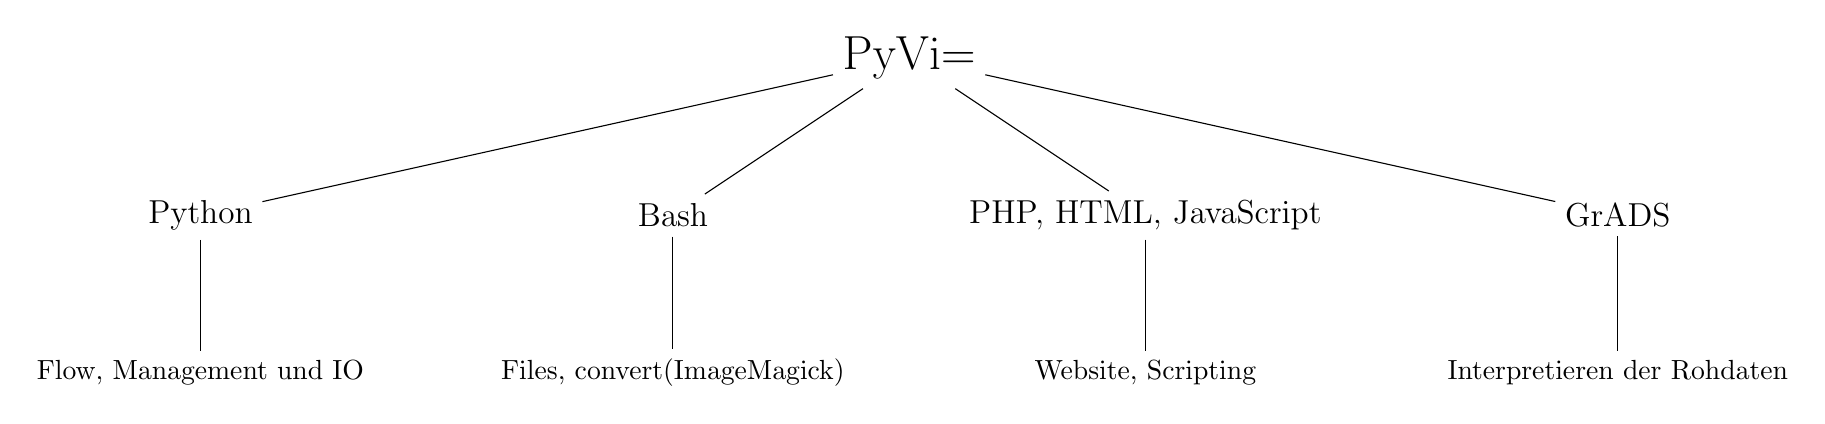
\begin{tikzpicture}[
every node/.style = {},
level 1/.style = {sibling distance = 6cm},
level distance = 2cm
]
\node {\LARGE PyVi$=$\vs}
    child { node {\large Python} 
    		child { node{Flow, Management und IO}}
    }
    child { node {\large Bash}
    		child { node {Files, convert(ImageMagick)}}
    }
    child { node {\large PHP, HTML, JavaScript}
    		child { node {Website, Scripting}}
    }
    child { node {\large GrADS} 
    		child { node{Interpretieren der Rohdaten}}
    };
\end{tikzpicture}
}
\end{center}
\label{fig:pyvi}
\caption{Benutzte Programmiersprachen}
\end{figure}

\subsubsection*{Hauptprogramm}
Das Hauptprogramm, gleichbedeutend mit der Main-Methode anderer Programmiersprachen
ist in Python das Modul, welches vom Interpreter aufgerufen wird. Dieses kann über
Importaufrufe weitere Module einbinden. So kann der Programmablauf übersichtlich doch
komplex sein.\\
Dieses Mainmodul ist die Datei auvi.py,
\lstinputlisting[language=Python,firstline=12, lastline=41,firstnumber=12,caption={,,Mainfunktion'' von \vs\ (auvi.py)}]{\pyvidir auvi.py}
diese Zeilen stellen die Definition der ,,Mainmethode'' dar. In ihnen wird auf größere
Methoden außerhalb der Datei zugegriffen. Durch diesen Aufbau ist es möglich die
Funktionalität der für diesen Zweck geschrieben Software zu erweiten oder für andere
Projekte zu benutzen.\\
Das Programm handelt grundsätzlich so, dass es erst die Dateistruktur um sich herum
aufbaut. Dafür greift es auf Funktionen aus dem Modul filemanager, in der Datei
filemanager.py zu. Dieses Verhalten bestand seit der ersten Version des Programmes wurde
aber durch die Übersetzung in Python von Bash wesentlich robuster und allgemeiner.\\
Nachdem einige Konstanten festgelegt werden, werden aus Dateien über andere Module
die vom Nutzer abgefragten Parameter, Orte und Gebiete ausgelesen. Diese Definitionen liegen
in JSON Form vor und können leicht von anderen Programmen geschrieben und gelesen werden.\\
Die richtige Arbeit des Programmes wird dann in verschachtelten for-Schleifen erledigt, in
denen über die verschienden Parameter und Orte iteriert wird.\\
\lstinputlisting[language=Python,caption={Hinzufügen von neuen Orten, Gebieten und Parametern (local.py)},firstline=11,lastline=28,firstnumber=11]{\pyvidir local.py}
Diese Methoden bieten ein Interface um von Außen neue Orte sowie Parameter
der Routine hinzuzufügen.
Sie geben zusätzlich dem Nutzer immer Feedback was gerade geschehen ist.
\lstinputlisting[language=Python,caption={Routine zum schreiben von JSON Dateien (local.py)},firstline=30,lastline=41,firstnumber=30]{\pyvidir local.py}
Diese Funtionen werden aufgerufen um die Pythonstrukturen in JSON Objekte umzuwandeln
und schließlich in eine Datei zu schreiben. Großgeschrieben Variablen aus
dem Quelltext stehen für vordefinierte,
konstante, Strings für Ordner- oder Dateibezeichnungen.\\
Über die folgenden Methoden können die geschrieben JSON Dateien dann ausgelesen werden.
\lstinputlisting[language=Python,caption={Datei In- und Output (filemanager.py)},firstline=39,lastline=66,firstnumber=39]{\pyvidir filemanager.py}
Die Methode createOutputDirs ist die Definition die aus der Mainmethode aufgerufen wird
um die Ordnerstruktur vorzubereiten. Die Grafiken werden in diese Ordnerstruktur geschrieben.
Eine wichtige Entscheidung musste getroffen werden wie die Daten gespeichert werden sollen,
damit gleichzeitig immer möglichst neue Daten angezeigt werden können, niemals Dateien nicht
vorhanden sind und trotzdem die Datenkapazität minimal gehalten werden soll.
Dieses Problem wurde so gelöst, dass die Grafiken in einen temporären Ordner geschrieben
werden und von dort aus sobalt sie alle fertig generiert wurden die alten Grafiken in
ihrem festen Speicherort überschreiben. Dies bedeutet für den Datenträger, dass maximal
zwei Sätze der Grafiken gespeichert werden müssen und es keine ,,Downtime'' auf dem
Server gibt, welche bedeuten würde das zeitweise Grafiken bestimmter Art nicht aufgerufen
werden können.
\lstinputlisting[language=Python,caption={Bewegen der Dateien (filemanager.py)},firstline=68,lastline=100,firstnumber=68]{\pyvidir filemanager.py}
Die einzelnen Schnappschüsse der Konturplots werden über die Methode convertToGifs zu
Gifdateien umgewandelt. Gifs sind animierte Grafiken, die wie Videos gut die zeitliche
Entwicklung der Konturplots darstellen.\\
Für Präsentationen oder Geräte welche Gifs nicht gut darstellen können kann über die
Funktion convertGifToMp4 die Gifdatei zu einer MP4 Datei umgewandelt werden.
Dafür wird aber die Bibliothek ffmpeg auf dem Rechner, welcher die MP4 Datei erstellen
will vorausgesetzt.

\subsubsection*{JSON Definitionen}
Im folgenden Listing wird die Definition von Ortspunkten
\footnote{Ortspunkte stehen im Kontrast zur Gebietsdefinition. Gebiete werden durch minimale Breiten- und Höhengrade definiert und besitzen eine Breite und Höhe. Anwendungsbeispiel: Europa, Welt, Asien, ...} gezeigt.
Diese werden im JSON Format gespeichert.
Die Liste kann um beliebig viele andere Orte erweitert werden.
\lstinputlisting[language=json, caption={Beispielobjekte für Ortspunkte (locals.json)}]{\pyvidir locals.json}
In der Liste steht der erste String für den Ortsnamen. Der zweite Wert ist ein Double für den Breitengrad gefolgt vom Längengrad.
Da von den Orten auch ein Konturplot erzeugt werden soll wird mit dem 4. Wert abgespeichert wie groß die Übersichtskarte sein soll (In Grad um den Ort).
Der letzte Wert zur Definition eines Ortspunktes ist die Zeitdifferenz zur GMT Zeit.\\
Diese Datei ist der ursprüngliche Grund für den Umstieg auf Python.
Python kann ,,out-of-the-box'' mit JSON Dateien umgehen. An der Definition kann man schon ablesen,
dass ein Hinzufügen des Ortes sehr leicht geschehen kann. Dafür muss dem Ort nur trivialerweise ein Name
gegeben werden, und dann ein Breiten- und Längengrad zugewiesen werden. Diese Informationen reichen
schon um die meisten Grafiken zu erzeugen, der Flächenparameter ist nur ein optischer Parameter und kann
ausgelassen\footnote{Der ,,Area''-Parameter muss auf 0 initialisiert werden,
weil um Speicherplatz zu sparen die Orte in einer
Python-list und nicht in einem Python-dict gespeichert werden} werden. Auch die Zeitzoneninformation kann
ausgelassen werden.

\subsubsection*{GrADS Scripte}
\lstinputlisting[language=grads,
caption={GrADS Routine zum erstellen allgemeiner Funktionsgraphen (line.gs)}]{\pyvidir grads/line.gs}
\lstinputlisting[language=grads,
caption={GrADS Routine zum erstellen allgemeiner Konturplots (plot.gs)},
label= code:plotgengs,
firstline=104, lastline=115, firstnumber=104]{\pyvidir grads/plot.gs}
In Listing \ref{code:plotgengs} greift das Programm auf verschiedene eigene
Funktionen zurück um die Konturplotgrafiken zu füllen.
Um den Ablauf des Programmes zu verstehen sind die wichtigsten Stellen hier aufgelistet und erläutert.
\lstinputlisting[language=grads,caption={Zeichnen der Achseneinteilung und Legende unter GrADS für Plots (plot.gs)}, firstline=117, lastline=136, firstnumber=117]{\pyvidir grads/plot.gs}
Die Variable $color$ spielt in diesem Teil des Skriptes eine große Rolle.
Diese Variable ist in diesem Kontext ein Pointer auf ein anderes GrADS Skript,
welches die Farbdefinitionen enthält.
Dieses Farbscript lässt sich leicht vom Computer nach den Eingaben eines Nutzers erzeugen.
\lstinputlisting[language=grads,firstline=8, lastline=28,caption={Beispiel Farbdefinition für Temperaturkonturplots (t2m.gs)},label=code:t2mcols]{\pyvidir grads/t2m.gs}
In Listing \ref{code:t2mcols} wird die Funktion gezeigt die bestimmten Zahlen eine Farbe zuweist.
Diese Farben sind im RGB Format codiert.
Die Definition ist so zu lesen:

\begin{lstlisting}[language=grads]
	'set rgb <num> <rot> <gruen> <blau>'
\end{lstlisting}

Die Farbwerte sind in einem Intervall von $0$ gar nicht vorhanden bis $255$ voller Kanal.
Um diese Farbwerte dann zu nutzen müssen diese noch den Wetterdaten zugewiesen werden.
Dieses geschieht unabhängig von den Einheiten im selben Script.
Auch hier kann der Text leicht von einem Computer generiert werden.
\footnote{Wenn in dieser Arbeit davon gesprochen wird, dass Eingabedaten vom Computer
generiert werden ist gemeint,
dass ein Nutzer der Website oder App seine Anfrage mithilfe einer HTML-Form abgibt
und aus diesen Werten im Hintergrund eine Datei erzeugt oder geändert wird.}


\subsubsection*{Webseite}
Das Front-End der Software ist eine Website
\footnote{Diese Website kann auch in eine App gepackt werden,
zur Veröffentlichung braucht man allerdings ein Entwicklerkonto bei Google oder Apple},
diese kann aber auch über eine Shell umgangen werden, indem man \vs direkt Befehle
übergibt und die Bilder serviert bekommt.\\
Die Website ist programmiert in HTML (Hyper Text Markup Language),
PHP (PHP\footnote{Rekursives Akronym}: Hypertext Preprocessor) und JavaScript.
Als Webserver wird Apache2 eingesetzt \cite{php} \cite{apache} \\
Der Server der diese Website ,,served'' ist nicht über eine Domain aus dem Internet
erreichbar, da sobalt Grafiken benötigt wurden später das gesammte Projekt auf
einen Rechner heruntergeladen wurde und von dort lokal ausgeführt wurde.
Die Website liest genauso wie \vs die JSON Dateien aus und kann aus den
Routinen schlussfolgern unter welchem Dateipfad die Grafiken nach der Generation
liegen müssen. Dann muss die Website nur noch auf die Grafiken verlinken.
Für die Projektarbeit wurde die Website hauptsächlich genutzt um das Arbeiten mit
dem Dateimanager zu minimieren, da dieser bei jedem Ordnerwechsel die Grafiken lud,
der Webbrowser allerdings erst auf Befehl die Grafiken lädt.


\subsubsection{Versionen}
Im Laufe der Arbeit entstanden mehrere lauffähige Versionen.
Diese beginnen mit puren GrADS-Scripten um überhaupt Grafiken
zu erzeugen zu Beginn der Projektarbeit in 2013.
Um dieses Erzeugen zu automatisieren wurden alle nötigen Befehle in eine BASH Datei verpackt.
Diese Bash Datei musste die Ordnerstruktur herstellen und kontrollieren.
Sie war außerdem in der Lage neue Versionen der Software auf einem Server zu erkennen
und auf Befehl vom Server zu laden und sich selbst zu ersetzen.
Auf diese Version baute das Projekt weiterhin auf,
nachdem sie bei dem Jugend Forscht Wettbewerb 2014
präsentiert wurde und den zweiten Platz erzielte.\\
Um allerdings schnellere Ergebnisse zu erzielen wurde
das komplette Programm von Bash in Python übersetzt.
Durch die modulare Struktur von Python können meine
Funktionen in andere Projekte als Bibliotek eingebunden werden.\\
Über Python kann man effektiver die Daten analysieren,
kann leichter komplexe Bedingungen kontrollieren und
auch die Interaktion mit dem Nutzer ist erleichtert
(z.B. durch das Nutzen von JSON Dateien).
Durch Python und JSON konnte man das Projekt dann vollständig automatisieren.
Zum Zeitpunkt der Arbeit wird GrADS noch immer Aufgerufen. Allerdings
wird durch die ständige Weiterentwicklung an einem neuen Projekt gearbeitet.
Dieses Projekt, ,,PilDap'' getauft soll von der GitHub Gemeinde mitentwickelt
werden und nativ in Python die selbe Aufgabe erfüllen wie GrADS \cite{pildap}.

\subsubsection*{Git}
Ab Anfang 2015 findet eine neue Umgebung anwendung um an
Programmen und der Setzung zu arbeiten.
Die Umgebung Git \cite{gitrepo}
ermöglicht im eigentlichen Sinne Programmierern gleichzeitig an
einem Projekt kooperativ zu arbeiten.
Die Umgebung konnte zuerst auf dem eigenen Server und später zusätzlich
auf der Website \link{GitHub.com} \cite{github} genutzt werden.
Der Git ,,Workflow'' ist auch ohne Internetverbindung komplett funktionstüchtig.
Ich mache Änderungen, verpacke sie und sende sie zum Server.
Dieses Änderungspacket erhält eine einzigartige Identifikation, eine SHA1 Hash \cite{gitsha1}.
Durch diese Identifikation kann man im Nachhinein auf jede einzelne Version
meiner Software und Setzung zugreifen. Wenn man also einen Fehler bemerkt kann man so
durch den Befehl $\text{git bisect}$ den Commit, d.h. die Änderung finden, die den Fehler
mit sich brachte.
Zusätzlicher erreicht man so eine hohe Datensicherheit \cite{linussaves} und schnelle parallele Entwicklung mit gegenseitiger Kontrolle\footnote{Ziel ist es den Inhalt zu kontrollieren, nicht die Kollegen}.

\subsubsection{genutzte Mittel} % AuVi Entwicklung
% Website, Server, ...
% Raspberry Pi x2
% Software: 	Linux -> Ubuntu, Debian, Raspbian
% 				Apache2, Git, Python2:3, PHP, SSH
% 				Editor SublimeText, Eclipse, Atom
AuVi wurde auf zwei Servern entwickelt. Einer als Entwicklungs- der andere als Integrationsserver.
Das hat zum Vorteil, dass jede Version mehrfach getested werden konnte.
Einer dieser Server ist ein Raspberry Pi mit den Betriebssystem Raspbian.
Der zweite Server wurde mehrfach verlegt und ist endlich auf der Platform travis-ci.org realisiert.
Bearbeitet wurde das Programm von offenen Betriebssystemen aus. Dazu zählen das schon genannte
Raspbian, eine Version von Debian, und auf unseren Laptops und PCs wurde hauptsächlich Ubuntu genutzt.
Zu den Programmen, welche die Projektarbeit ermöglichten zählen: Apache2 als Server
Software, Git als SCM\footnote{Source Code Manager oder Software Configuration Management},
Python2, Python3 und PHP als Programmiersprache, nautilus als Dateimanager für FTP und SFTP, sowie
SSH als Netzwerk-Shell.\\
Als Editor wurde zuerst SublimeText genutzt um die Bash- und später Pythondateien zu bearbeiten.
SublimeText wurde zwischenzeitlich durch Eclipse ersetzt um eine vollwertige IDE für PHP und Java zu
genießen. Die \LaTeX Dateien wurden anfangs aus dem selben Grund mit TexMaker bearbeitet.
Nachdem im Projekt weitere automatisierte Integrationsfortschritte gemacht wurden konnte auf
diese IDEs verzichtet werden, und es wurde nur noch auf den offenen Texteditor Atom zurückgegriffen.
Alle Linker- und Compileraufgaben der IDE wurden über Makefiles realisiert um die Spiegeln der
Entwicklungsumgebung auf ein Minimum von zwei Zeilen zu bringen. Ein Entwickler kann mit den
Befehlen $\text{git clone https://github.com/tibyte/auvi-hub}$ und $\text{make}$ seine Entwicklungsumgebung
so vorbereiten, dass er direkt den Stand der Software sieht und sie zugleich sofort einsetzbar ist.
Durch diese Optimierung kann ein Projektteilnehmer durch genau diese zwei Befehle seine Entwicklungsumgebung
in Sekunden einrichten.\\
Nachdem der beschriebene Aufbau lauffähig war griff das ,,Never touch a running System'' Prinzip.
Das AuVi-System wird als Black-Box behandelt, von dem erwartet werden kann, dass es auf anfragen
richtig reagiert und Änderungen dieses Verhalten nicht abändern.\\
Dieses Verhalten wird in der Branche als Feature-Freeze\footnote{Keine neuen Funktionen}
eines API-Levels\footnote{Version eines Programmes, welche sich untereinander um Patches unterscheiden,
aber kompatibel sind} \cite{semver} bezeichnet.\\
Für den Entwickler steht somit fest, dass die Software ihre Aufgabe erfüllt, aber noch optimiert
werden muss.

\subsubsection{Datenformate} % AuVi Schnittstelle
Da die erzeugten Grafiken auf einer Website und App dargestellt werden sollen
musste sehr darauf geachtet werden,
dass die Dateiformate zum einen komprimiert genug sind
um heruntergeladen werden zu können und zum anderen
noch einen gewissen Qualitätsstandard erfüllen.\\
Außerdem sind Mobiltelefone nicht in der Lage alle
Dateiformate anzuzeigen,
die ein Webbrowser auf einem Computer ohne Probleme handhabt.\\
Die Grafiken selbst werden im JPG oder PNG Format erzeugt, welches
Format genutzt wird entscheided GrADS autonom. Diese Grafiken werden
über ImageMagick zu GIF Dateien konvertiert. GIFs sind zwar nicht stark
komprimiert, können aber auf jedem Gerät abgespielt werden.
Falls man Speicherplatz sparen will oder die Animation wie ein Video nutzen will
werden die GIFs sofern ffmpeg installiert ist auch noch zu MP4 Dateien konvertiert.

\subsubsection{Schulhompage} % AuVi Schnittstelle
Da Jugend Forscht unter der Leitung von Herr Doktor Eixmann
ein Projekt des Schulzentrum Kühlungsborns ist
(\link{http://www.schulzentrum-kborn.de}) dieses Projekt auf der Schulhompage
unter ,,Lernen über Fächergrenzen'' als Campus Pro Projekt vertreten \cite{szkb}.
Dort ist dieses Projekt unter dem Titel ,,CaP \jf : Junge Atmosphären-forscher JAF'' aufzufinden.
Da die Bearbeitung der offiziellen Schulzentrum Kühlungsborn Seite sich als Umständlich aufzeigte,
wurde eine eigene Seite auf einem privaten Server eingerichtet.
Diese ist unter \link{http://team.viwetter.de}
für die Öffentlichkeit zu erreichen.
Diese Seite soll nicht die Ergebnisse des AuVi Programms
widerspiegeln sondern dient als Webpräsenz der Projektarbeit.

\subsection{Szenario} % AuVi
Da diese Visualisierungssoftware als Open Source Projekt angeboten wird kann der Nutzer
sie beliebig bearbeiten, in diesem Abschnitt werden einige Szenarien aufgezeigt wie das System
so wie es ausgeliefert wird genutzt werden kann.
Es gibt darüber hinaus sehr viele Möglichkeiten aus dem Programm individuellen Nutzen zu ziehen.
Python Entwickler können so diese Software als Bibliothek im Quelltext einbinden oder direkt den Quelltext
weiterentwickeln.

\subsubsection{Frühwarnung} % AuVi Szenario
Das entstandene System kann verwendet werden um
wetterbedingte Gefahrensituationen frühzeitig zu erkennen.
Anhand der globalen Datenquellen und dem Hintergrund des
Systems ist es einem Nutzer möglich für seinen Ort selbst die
Parameter zu wählen die für Ihn zum Beispiel eine Gefährdung darstellen.\\
Es ist wichtig, dass die Visualisierungen keine Laien abschreckten,
deshalb kann die Frühwarnung in Form eines
Ampelsystems an den Nutzer gebrach werden.
Dieser kann bei Interesse an der Frühwarnfunktionalität eine Spanne angeben,
in der der entsprechende Parameter sicher ist (grün),
gefährlich wird (gelb) oder gefährlich ist (rot).
Diese sehr visuelle Form soll dabei auf einem Blick ermöglichen die Wetterlage abzuschätzen.\\
Für detaillierte Auswertungen kann man andere Anzeigeformate wählen.

\subsubsection{Exotische Orte} % AuVi Szenario
Ob mitten im Ozean oder in der Wüste, das Programm liefert Prognosen für jeden Ort.
Die wichtigste Information die das Programm zum Ort brauche ist die Koordinatendarstellung des
Ortes auf dem Gradnetz der Erde.
Diese Darstellung besteht aus Längen- und Breitengrad (engl. Longitude, Latitude).
Das heißt jeder Ort kann durch das Intervall der Längengrade $[-180:180]$ und
der Breitengrade $[-90:90]$ dargestellt werden.
Es gibt aber, da das Gradnetz die Erde als mathematisches Objekt abstrahiert,
durch die reine Komplexität der Erdoberfläche und Form bei der Bestimmung der
Koordinaten Abweichungen \cite{tomgeo}.
Die Genauigkeit ist zudem von der Zeitspanne und
der Entfernung zur physikalischen Messstation abhängig.
Je weiter das Wetterereignis oder die Wetterprognose in der Zukunft liegt,
desto geringer ist dessen Genauigkeit.
Die Genauigkeit steigt, wenn sich eine Messstation im näheren Umfeld befindet und
nur eine kürzere Prognose verlangt wird.\\
Der Nutzer selbst hat viele Möglichkeiten die Koordinaten für den Ort seines Interesses herauszufinden.
Wenn er sich dort befindet kann jedes mobile Gerät oder Handy die Koordinaten ausgeben, außerdem kann
über ein Interface zu Google Maps ein Ort direkt ausgewählt werden.

\subsubsection{Wissenschaft} % AuVi Szenario
Wissenschaftler können von der Datenquelle bereitgestellte Parameter kombinieren
und sich so neben allgemein komplexeren meteorologischen Daten
auch für sie besonders interessante meteorologische Ereignisse grafisch darstellen lassen.
Wenn jemand zum Beispiel Zusammenhänge zwischen der Ozonschicht und der Temperatur erforscht,
kann er sich eine Grafik ausgeben lassen, die ihm diese beiden Parameter darstellt.
% Dr. Eixmann fragen, was man sich wissenschaftlich visualisieren könnte
\begin{center}
	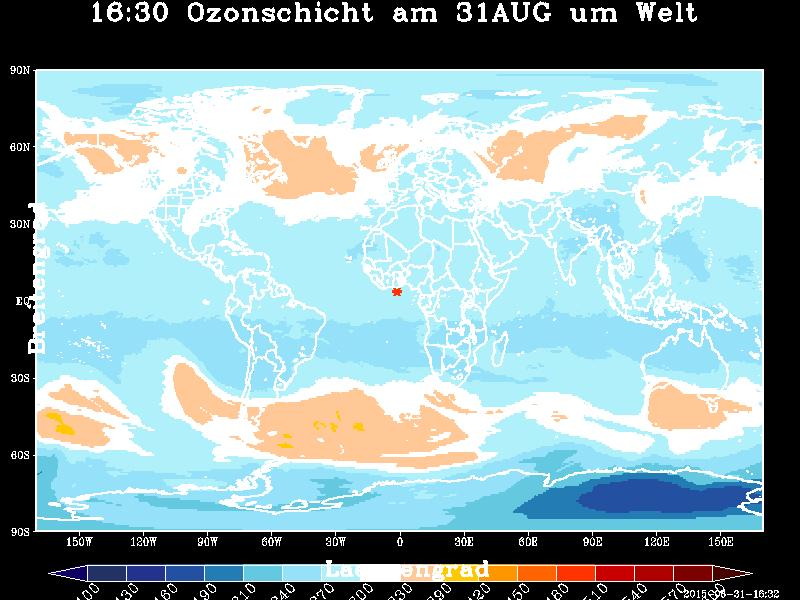
\includegraphics[width=\linewidth]{imgs/gl/to3_0013.jpg}
\end{center}

\subsubsection{Anpassung} % AuVi Szenario
Wie zuvor genannt kann der Nutzer eigene Muster einstellen und so das Programm erweitern.
Diese Möglichkeit erlaubt dem Nutzer diesen Service,
der angeboten wird, um eigene Funktionen zu erweitern.
Ein Beispiel ist der Segler, der in einem Bestimmten
Intervall von Windstärke und Windrichtung am besten seinen Sport ausüben kann.\\
Der Segler würde sich diese Parameter dann für das Gebiet seiner
Interesse plotten lassen und kann dann noch Farben wählen.
Ähnlich wie das Frühwarnsystem kann er sich nun aber
seine eigene Skala der ,,Eignung zum Segeln'' erstellen.
% TODO Verschiede Visualisierungen (der selben Daten)

\subsection{Öffentlichkeitsarbeit} % AuVi
% Messen, Vorträge, Dokumentation, Poster
% TODO Remove ,,Ich''s
Um diese Arbeit zu präsentieren, entstanden im Laufe des Projekts mehrere Poster.
Anfangs wurden diese in PowerPoint entwickelt, später wurde ein Umstieg
auf Gimp umgestiegen notwendig,
da sich Gimp für die Arbeit vorteilhafter gestaltete.
Auf den Postern war meist zuerst eine kleine Einführung in das Projekt.
Danach schloss sich eine nähere Erläuterungen desselben an.
Um das Poster für den Betrachter attraktiver und anschaulicher zu machen,
wurden einige Themen in grafischer Form dargestellt und
veranschaulichten so die Ergebnisse mit Beispielgrafiken. \\
Häufig wurde auch eine schriftliche Erläuterung des Projekts gefordert,
in der alles ausführlich erklärt wird.
Diese Dokumentation des Projekts wurde in \LaTeX gesetzt.
Auch in diesen Dokumentationen wurden Übersichten und Grafiken als Anschauungsmaterial
beigefügt und nötigenfalls näher erläutert.\\
Solche Dokumentationen und Poster kamen zum Beispiel bei
den Landeswettbewerben \jf in Rostock (Mecklenburg Vorpommern) zur Anwendung.
Bei diesem Wettbewerb werden aus dem gesamten
Bundesland Projekte aus verschiedenen Fachgebieten präsentiert.
Es wird unterteilt in Arbeitswelt, Biologie, Chemie,
Mathematik/Informatik, Geo- und Raumwissenschaften und Technik.
Die jeweils Erstplatzierten in jedem Bereich
qualifizieren sich für den darauffolgenden Bundeswettbewerb.
Die Teilnahme am Jugend Forscht Wettbewerb begann erstmalig 2013.
,,Auvi - Automatisierte Visualisierung von Wetterstations- und Wetterprognosedaten''
erreichte den zweiten Platz in der Kategorie Geo- und Raumwissenschaften des Wettbewerbes
Jugend Forscht 2014.
Im Jahr 2015 erreichte das weiterentwickelte
,,AuVi - Automatisierte Visualisierung von meteorologischen Daten''
die Qualifizierung für den Bundeswettbewerb.\\
Veranstaltungen bei denen das Projekt vorgestellt wurde war zum Beispiel der IHK-Schulpreis.
Im Jahr 2014 bewarb sich das Schulzentrum Kühlungsborn mit dem Projekt CampusPro.
Mit Vertretern aus anderen Projekten der Schule wurde das Schulzentrum hier vertreten.
Im Jahr darauf trat das Projekt ,,Auvi'' alleine an.\\
Am Schulzentrum Kühlungsborn wird die Möglichkeit geboten durch
umfassende Projektarbeit ein IHK-Zertifikat zu erlangen.
Um dieses zu erlangen werden Vorträge gehalten, in denen das jeweilige Projekt präsentiert wird.
Im Jahr 2014 wurde solch eine Vortragsveranstaltung durch einen Vortrag zum Thema ,,Auvi'' eröffnet.
Dies war eine kurze Vorstellung des Projektes.
